\chapter{Grundlagen}
\section{Usability}
\textit{Usability} in der Software-Entwicklung ist ein Qualitätsmaß, anhand dessen eine Einschätzung über die Einfachheit der Bedienung einer Benutzeroberfläche ermöglicht wird \cite{Nielsen2012}. Umgangssprachlich wird der Begriff \enquote{Benutzerfreundlichkeit} als deutsches Synonym verwendet. Betrachtet man jedoch den Wortstamm genauer, bemerkt man, dass die englische Vokabel aus zwei einzelnen Wörtern besteht. Dies ist zum einen \enquote{use} (engl. benutzen) und zum anderen \enquote{ability} (engl. die Möglichkeit). 

Nach Nielsen wird die Qualität einer Anwendung hinsichtlich der Usability durch 5 Kernaspekte bestimmt:
\begin{itemize}
	\item Erlernbarkeit
	\item Effizienz
	\item Einprägsamkeit
	\item Fehlertoleranz
	\item Zufriedenheit \cite{Nielsen2012}
\end{itemize}
Alle diese Aspekte können zu einer guten Gebrauchstauglichkeit beitragen. Eine hohe Erlernbarkeit ist gegeben, wenn der Dialog zwischen der Maschine und dem Anwender einfach gestaltet ist, sodass die Bedienung schnell erlernt werden kann. Es ist hilfreich, Designkonzepte zu verwenden, die dem Anwender aus anderen Anwendungen oder aus der Natur vertraut sind \cite[Learnability]{UsabilityFirstGlossary}. Auch die Erfüllung psychologischer Grundsätze (siehe Kap. \ref{sec:uxdPsychology} und Kap. \ref{sec:uidRules}) ist ein wichtiger Faktor. Ein effizienter Dialog erlaubt es dem Nutzer, seine Ziele möglichst schnell zu erreichen. Kurze Ladezeiten und wenige zur Problemlösung benötigte Interaktionen fördern die Effizienz. Einprägsam ist eine Software, wenn ein Nutzer nach längerer Nicht-Benutzung dieser, ohne viel Zeitaufwand, den professionellen Umgang damit wieder erlernen kann \cite{Nielsen2012}. Bei der Fehlertoleranz geht es darum, dass die Anwendung fehlerhafte Eingaben erkennt und behandeln kann. Entweder kann die Anwendung den Fehler kompensieren und bereinigen oder der Nutzer muss über die Fehleingabe informiert werden und die Gelegenheit bekommen, korrekte Eingaben zu machen. Da bei der Usability stets der Nutzer im Fokus der Entwicklung steht, ist es von entscheidender Bedeutung, diesen zufrieden zu stellen. Ein gutes Design, das eine angenehme Bedienung ermöglicht, hilft dabei \cite{Nielsen2012}. \par

\section{User-Experience Design} \label{sec:uxd}
Der Begriff \textit{User-Experience} (kurz: UX) beschreibt das Nutzungsempfinden einer Person, wenn Sie mit einem System interagiert. Der Ausdruck ist meist im Bereich der Mensch-Computer-Interaktion vorzufinden, beschränkt sich aber nicht auf diesen. \cite{Gube2010} So kann der Begriff auch auf andere Produkte, wie z.B. Mikrowellen, Brettspiele oder ganze Produktreihen (vgl. Microsoft Office Produkte) angewandt werden. Im Rahmen dieser Arbeit wird jedoch nur der Teilbereich der Mensch-Computer-Interaktion im Rahmen einer einzelnen Anwendung betrachtet. \par
Im Gegensatz zur Usability berücksichtigt die UX die Erwartungshaltung des Nutzers und versucht, ein angenehmes Gesamtbild der Anwendung und der Interaktion mit dieser zu vermitteln. Das Ziel des User-Experience Designs ist es nicht nur, eine hohe Produktivität zu ermöglichen, vielmehr versucht sie, die Interaktion zu einem Erlebnis zu machen, das dem Anwender positiv in Erinnerung bleibt. Dies geht sogar so weit, dass der UX-Designer beschließt, dem Nutzer unter Umständen Funktionalitäten vorzuenthalten, um das Erlebnis zu sichern \cite{Thielsch2015}. Als Beispiel führt Thielsch den \textit{Drift-Table} an. Bei dem Drift-Table handelt es sich um einen niedrigen Couchtisch, in dem ein Bildschirm eingebaut wurde, der Luftaufnahmen von Großbritannien zeigt. Durch Kraftausübung an den Kanten des Tisches kann über das Land mit einer mäßigen Maximalgeschwindigkeit (50 km/h) \enquote{gereist} werden. Obwohl sich viele Nutzer gewünscht haben, direkt zu einem Ort springen zu können, hat sich der Erfinder bewusst dagegen entschieden, um das Erlebnis zu wahren \cite{Thielsch2015}. \par

\subsection{Interaktionsdesign} \label{sec:interactionDesign}
Ein Teilgebiet des UX-Designs ist das Interaktionsdesign (kurz: IxD). Der Fachbereich beschäftigt sich konkret mit den Schnittstellen, die ein Computersystem zwischen der Maschine und dem Nutzer bietet. Über diese Eingabe- und Ausgabesysteme können Informationen in beide Richtungen ausgetauscht werden.\par
Dafür muss der Benutzer sich zunächst darüber im Klaren sein, welches Ziel er mithilfe der ihm gegebenen technischen Möglichkeiten verfolgt. Er überlegt sich Handlungsschritte, von denen er glaubt, dass sie ihn zu seinem Ziel führen. Bei der Ausführung dieser, interagiert er mit dem Computersystem, welches die Eingaben verarbeitet und die Anwendung in einen neuen Zustand überführt. Dieser neue Zustand, der sich z.B. in einer Änderung der grafischen Oberfläche bemerkbar macht, wird von dem Nutzer interpretiert, woraufhin dieser einen weiteren Handlungsschritt ausführt. Dies tut er solange bis er seine Zielsetzung erreicht hat \cite{Ullenboom2014}. Daraus ergibt sich das Konzept einer Interaktion. \enquote{Das Ziel des Interaktionsdesigns ist es nun, diese Interaktion so zu gestalten, dass der Benutzer möglichst effizient, effektiv und zufriedenstellend an seine Ziele kommt\cite[S. 122]{Ullenboom2014}}.\par
Ein konkretes Beispiel ist das Ausdrucken eines Dokumentes in Schwarz-Weiß. Der Nutzer wählt aus dem Menü den Befehl \textit{Drucken} aus. Daraufhin öffnet sich ein Fenster, in dem die Einstellungen spezifiziert werden müssen. Der Anwender bekommt diese visuelle Änderung mit und überlegt sich, wo er welche Einstellungen ändern kann. Er wählt in der aktuellen Ansicht den zu verwendenden Drucker aus und betätigt daraufhin die Schaltfläche zum Verwalten der Druckereinstellungen. In dem weiteren Fenster kann er nun die Farbe auf Schwarz-Weiß stellen. Er bestätigt die Änderung und sendet danach den Druckauftrag ab. Werden keine Fehler festgestellt, ist damit die Interaktion abgeschlossen.\par
Donald A. Norman hat ein Modell entwickelt, das eben diese Interaktion abbildet. Es besteht aus 7 Phasen, die der Nutzer durchläuft, wenn er mit einem System interagiert. \par
% Grafik
Um diesen Interaktionsverlauf zu gewährleisten und die Probleme zu minimieren, definierte Norman 6 Designprinzipien:
\begin{itemize}
	\item \textbf{Sichtbarkeit:} Wichtige Funktionen sollten für den Nutzer auf Anhieb sichtbar sein
	\item \textbf{Feedback:} Das System sollte nach einer Aktion sofort eine Rückmeldung geben
	\item \textbf{Einschränkungen:} Im aktuellen Zustand unzulässige Funktionen sollten ausgeblendet oder eindeutig erkennbar deaktiviert werden
	\item \textbf{Aktion und Wirkung:} Für jedes Interaktionselement sollte klar erkennbar sein, wie und worauf es sich auswirkt
	\item \textbf{Konsistenz:} Für identische Interaktionen sollten immer die gleichen Bedienelemente verwendet werden
	\item \textbf{Affordance:} Objekte sollten durch ihre Gestalt (Form, Farbe, etc.) eine Selbsterklärungsfähigkeit besitzen \cite{Ullenboom2014}
\end{itemize}
\subsubsection{Eingabegeräte} \label{sec:inputDevices}
\heading{Maus}

\heading{Tastatur}

\heading{Touch}

\section{Visual Design} \label{sec:uid}
\textit{\enquote{Das Visual Design beschäftigt sich mit der Gestaltung einer Benutzeroberfläche \cite[S. 182]{Ullenboom2014}.}} Es baut auf den Beschlüssen in der Phase des Interaktionsdesign auf und verleiht der Oberfläche ihre finale Gestalt.\par
Der Visual Designer kümmert sich dabei um die Erstellung von prototypischen Designvorschlägen, die unter Anwendung von Designgrundlagen und -richtlinien entstehen. Das Ziel hierbei ist es, ein Konzept zu erstellen, das zugleich den Nutzer anspricht und zusätzlich die Usability durch Beachtung oben genannter Grundsätze verbessert. Im Laufe des Prozesses werden Objekte so platziert und gestaltet, dass eine einfache Orientierung möglich ist. Durch Farbkonzepte, basierend auf Erkenntnissen der Farbpsychologie, kann die Aufmerksamkeit konkret auf bestimmte Elemente gelenkt und Emotionen ausgelöst werden (durch Assoziation von Farben mit Elementen der Realität). Weitere Themengebiete sind Typographie, also das Auswählen von Schriftform, -größe, etc. und das Erstellen von Grafiken, Symbolen und Piktogrammen. \cite[S. 182]{Ullenboom2014}.

\subsection{Gestaltgesetze} \label{sec:uidRules}
Bei den Gestaltgesetzen handelt es sich um neuropsychologische Grundsätze, nach denen Objekte vom Menschen wahrgenommen und interpretiert werden. Berücksichtigt man diese Gesetze beim Design von Benutzeroberflächen, lassen sich Wahrnehmungseffekte auf subtile Weise erzeugen. Zum Beispiel kann die Aufmerksamkeit des Nutzers verstärkt auf gewisse UI-Elemente gelenkt oder die Bedienung vereinfacht werden. Nichtbeachtung dieser Regeln kann zu einer chaotisch wirkenden Benutzeroberfläche führen. Die wichtigsten Gestaltgesetze sind folgend aufgeführt.\par
\heading{Gesetz der Nähe}
\textit{\enquote{Objekte, welche nahe beieinander liegen, werden vom Auge gruppiert \cite[S. 186]{Moser2012}.}}\par
\begin{figure}[H]
 \centering
 
\includegraphics[width=0.25\textwidth]{grafiken/Gesetz_Naehe.png}
 \caption{Gesetz der Nähe \cite{Schossmann}}
 \label{fig:gesetzNaehe}
\end{figure} 
Durch Verringern der Abstände oder Vergrößern der Weißräume zwischen UI-Elementen, kann bewusst eine Gruppierung eingeführt werden, ohne dass zusätzliche Trennlinien oder Container von Nöten sind \cite[S. 186]{Moser2012}.\par
\heading{Gesetz der Ähnlichkeit}
\textit{\enquote{Visuell ähnliche Objekte werden vom Auge gruppiert \cite[S. 187]{Moser2012}.}}\par
\begin{figure}[H]
 \centering
 
\includegraphics[width=0.25\textwidth]{grafiken/Gesetz_Aehnl.png}
 \caption{Gesetz der Ähnlichkeit \cite{Grigo}}
 \label{fig:gesetzAehnl}
\end{figure} 
Schaltflächen können auch durch Verwendung verschiedener Formen, Farben oder Größen voneinander abgegrenzt und gruppiert werden. Besonders bei der Visualisierung von Datenbeständen in Diagrammen (Farbe und Form der Datenpunkte und der Legende) ist diese Eigenschaft hilfreich \cite[S. 187]{Moser2012}.\par
\heading{Gesetz der Prägnanz}
\textit{\enquote{In einer Vielzahl von Objekten werden diejenigen zuerst wahrgenommen, welche sich durch ein oder mehrere Merkmale vom Rest abheben \cite[S. 187]{Moser2012}.}}\par
\begin{figure}[H]
 \centering
 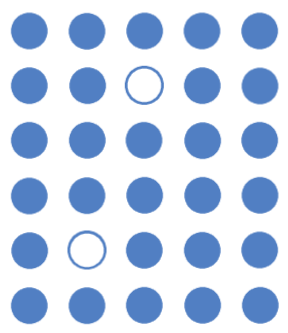
\includegraphics[width=0.25\textwidth]{grafiken/praegnanz.png}
 \caption{Gesetz der Prägnanz}
 \label{fig:gesetzPraeg}
\end{figure}
Ist ein Element oder eine Information \enquote{besonders} dargestellt, wird sie als erstes wahrgenommen. So können wichtige Informationen oder Bedienelemente hervorgehoben werden.\par
\heading{Gesetz der Kontinuität}
\textit{\enquote{Dieses Gesetz besagt, dass zum Beispiel Linien an Schnittpunkten eher als Fortführung ihrer bisherigen Linienführung, denn als eine Richtungsänderung gesehen werden \cite{Grigo}.}}\par
\begin{figure}[H]
 \centering
 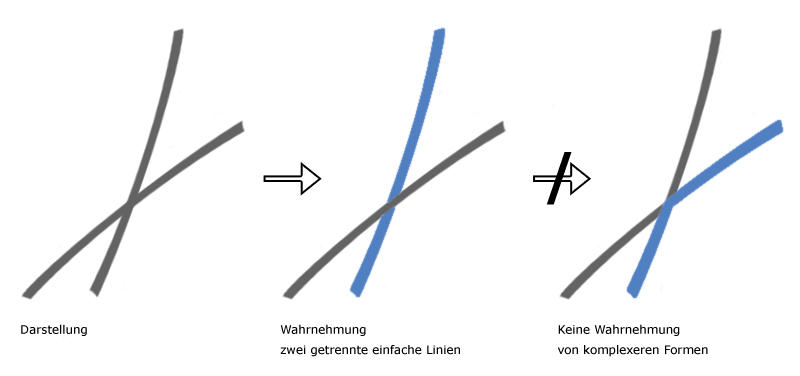
\includegraphics[width=0.8\textwidth]{grafiken/kontinuitaet.png}
 \caption{Gesetz der Kontinuität \cite{Grigo}}
 \label{fig:gesetzKonti}
\end{figure}
Elemente mit sanften Konturübergängen werden eher als Einheit erkannt als Elemente mit harten Übergängen \cite{Moser2012}.  Dies lässt sich unter anderem auf die Textorientierung anwenden. Sind mehrere Textzeilen nacheinander links orientiert, werden sie als zusammengehörig empfunden. Folgen daraufhin rechtsbündige Zeilen, bilden diese eine eigene Gruppe.\par
\heading{Gesetz der Geschlossenheit}
\textit{\enquote{Unser Auge komplettiert fehlende Teile einer Figur automatisch. \cite[S. 187]{Moser2012}.}}\par
\begin{figure}[H]
 \centering
 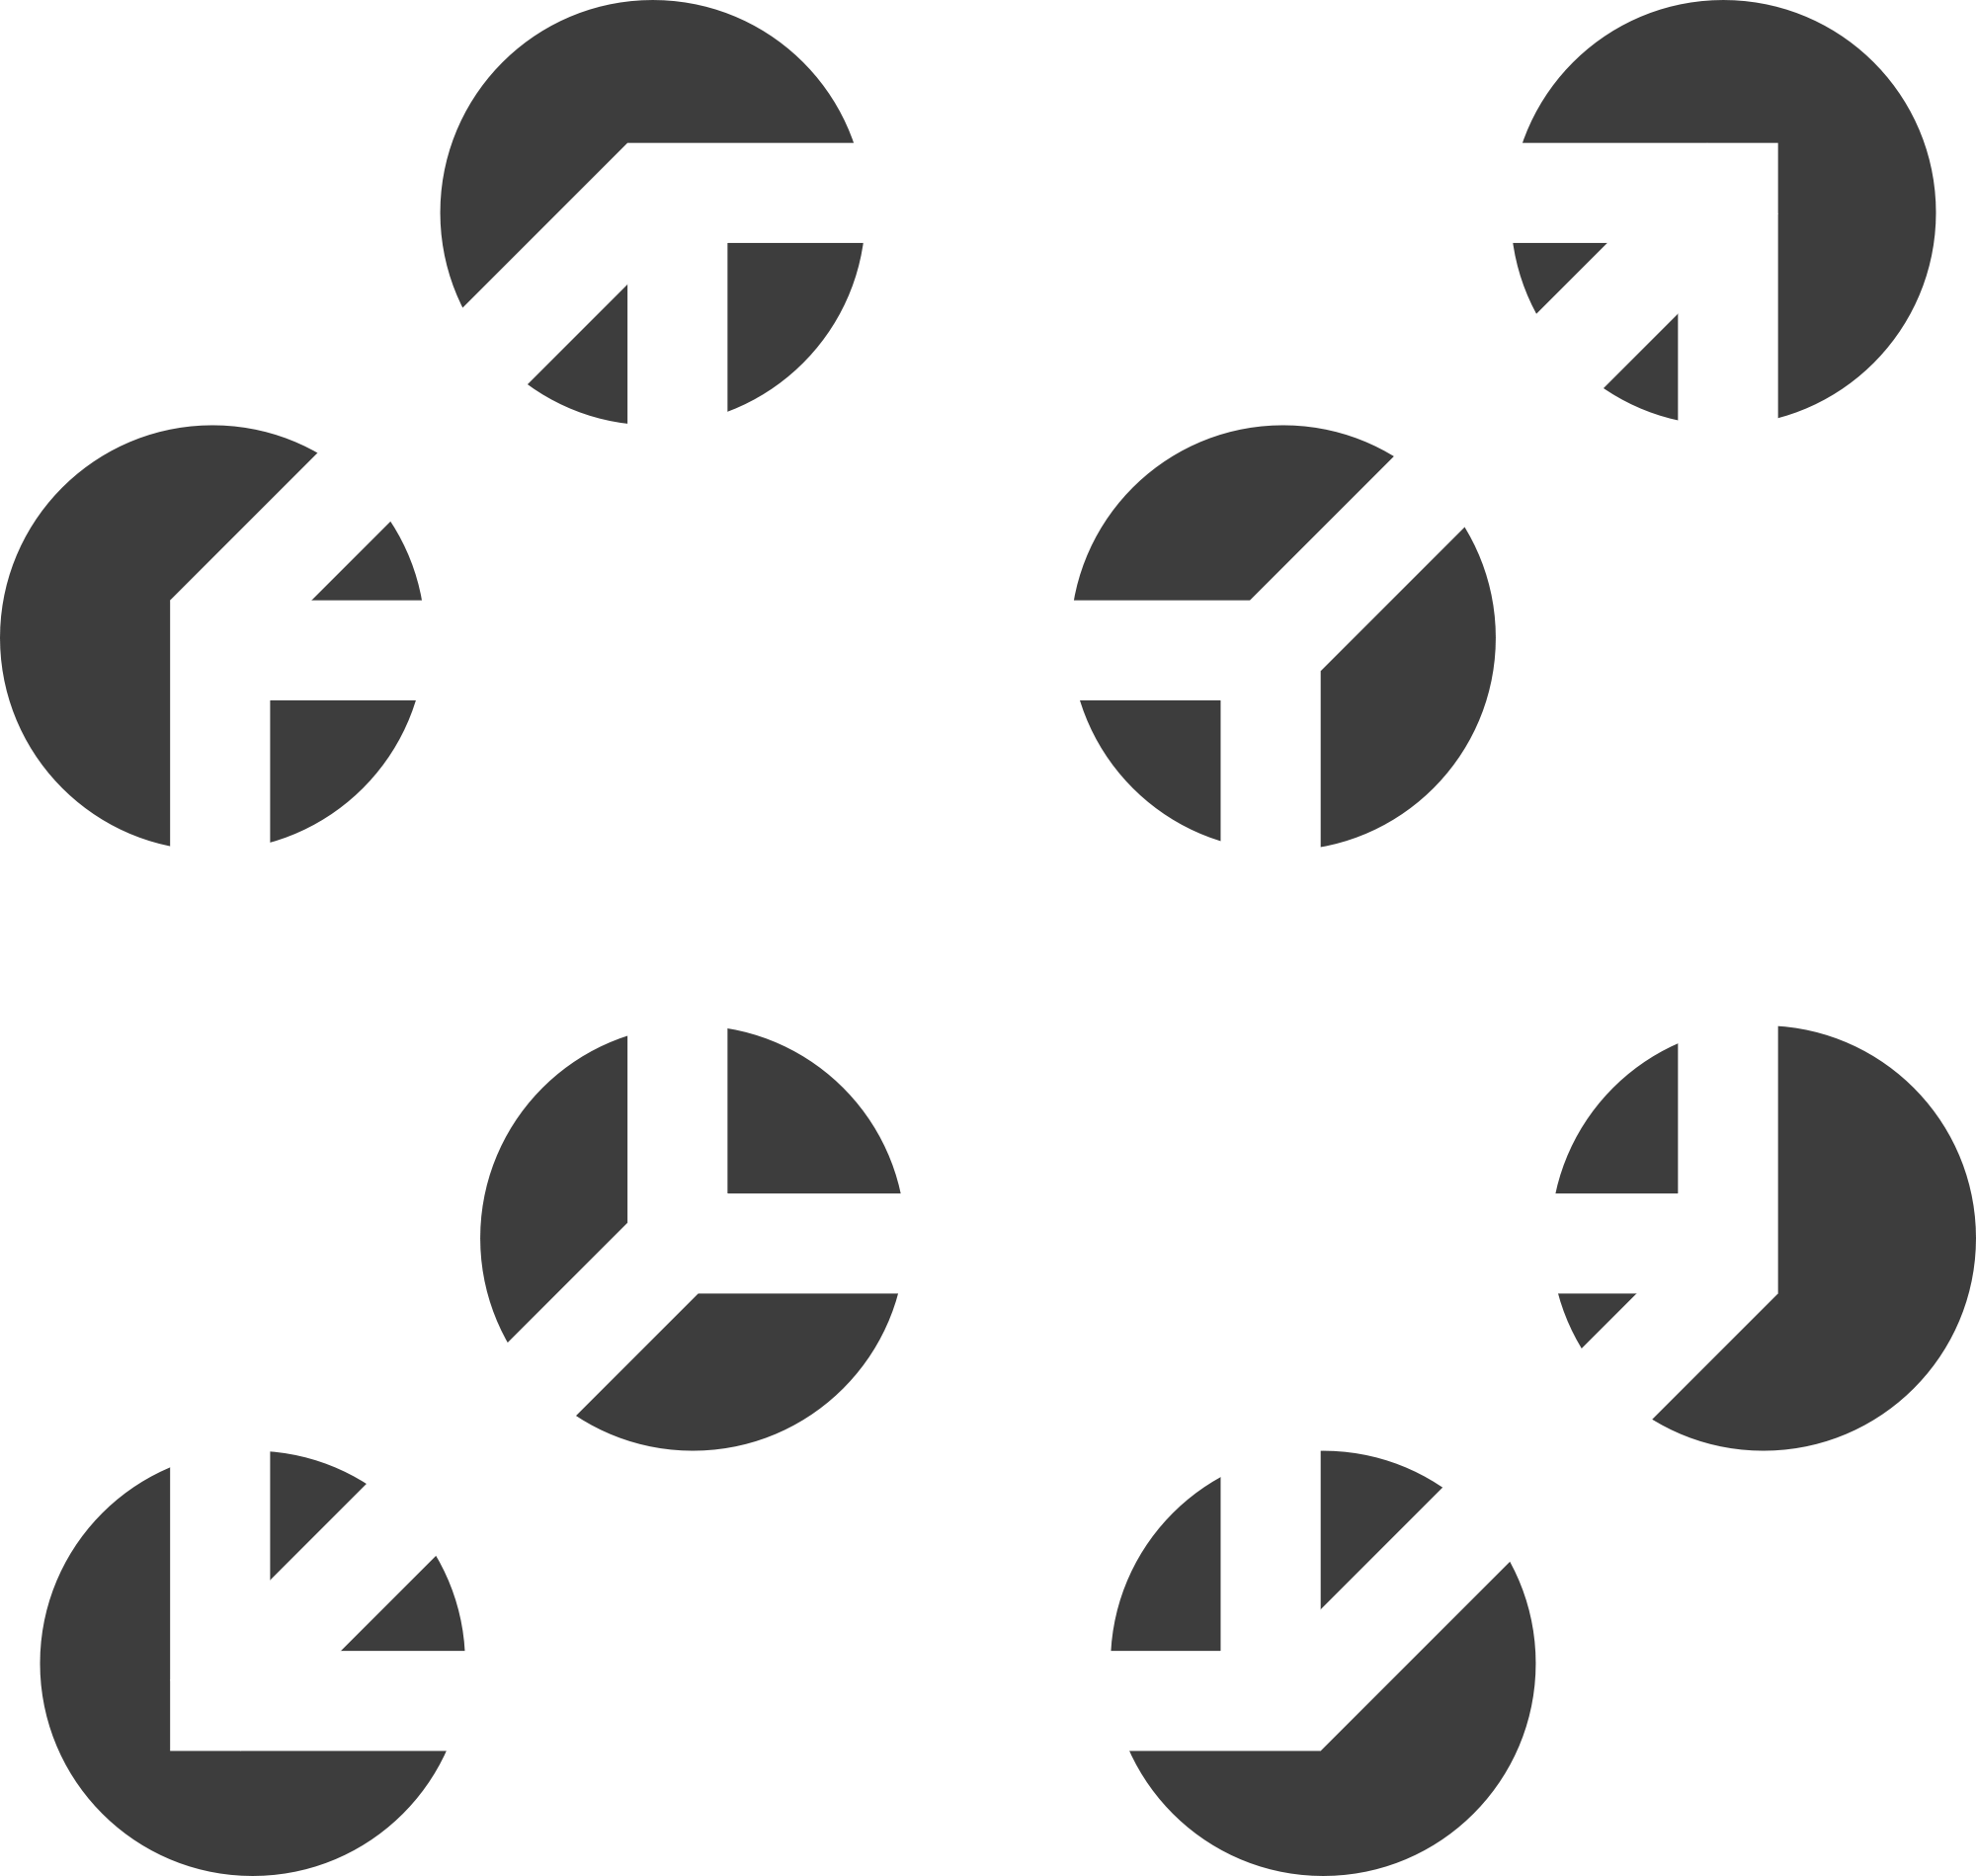
\includegraphics[width=0.25\textwidth]{grafiken/geschlossenheit.png}
 \caption{Gesetz der Geschlossenheit \cite{WikiGestaltgesetze}}
 \label{fig:gesetzGeschloss}
\end{figure}
Das Gesetz der Geschlossenheit kann dazu dienen, die Komplexität von Bedienelementen zu reduzieren, indem Teile davon weggelassen werden. Die fehlenden Bereiche werden durch die Wahrnehmung automatisch ergänzt. Dieser Effekt funktioniert jedoch nur bei dem Nutzer bekannten Formen \cite{Moser2012}.\par
\heading{Gesetz des gemeinsamen Schicksals}
\textit{\enquote{Wenn sich mehrere Objekte gleichzeitig oder in die gleiche Richtung bewegen, so werden sie als zusammengehörig empfunden \cite[S. 187]{Moser2012}.}}\par
\begin{figure}[H]
 \centering
 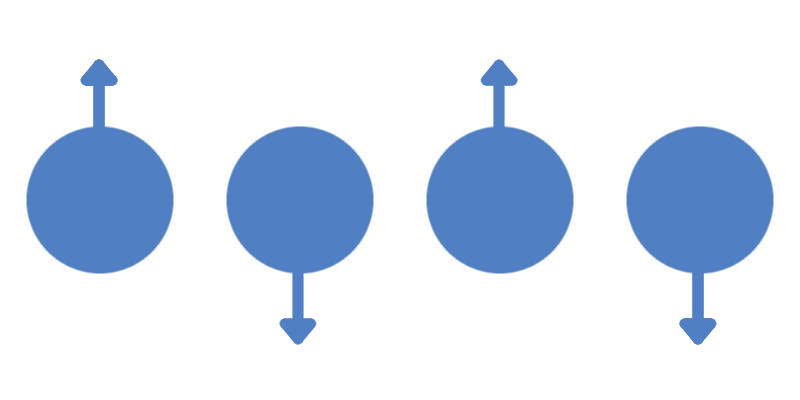
\includegraphics[width=0.2999\textwidth]{grafiken/schicksal.png}
 \caption{Gesetz des gemeinsamen Schicksals}
 \label{fig:gesetzSchicksal}
\end{figure}
Durch gleichzeitige bzw. gleichgerichtete Animation kann die Zusammengehörigkeit von Objekten erklärt werden \cite{Moser2012}. Unterschiedliche Animationen zur gleichen Zeit können dazu genutzt werden, die Unabhängigkeit verschiedener Gruppen zu betonen. In Abbildung \ref{fig:gesetzSchicksal} bspw. werden die sich nach oben und die sich nach unten bewegenden Elemente jeweils als eine Gruppe wahrgenommen.
\heading{Gesetz der gemeinsamen Region}
\textit{\enquote{Elemente in abgegrenzten Gebieten werden als zusammengehörig empfunden \cite{WikiGestaltgesetze}.}}\par
\begin{figure}[H]
 \centering
 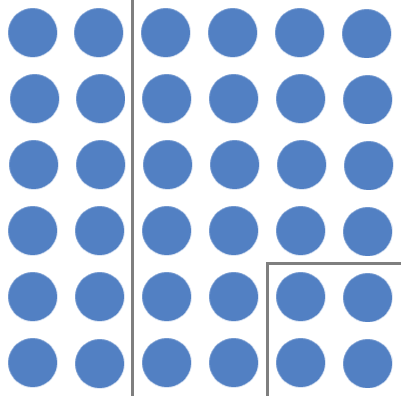
\includegraphics[width=0.25\textwidth]{grafiken/region.png}
 \caption{Gesetz der gemeinsamen Region}
 \label{fig:gesetzRegion}
\end{figure}
Die wohl trivialste Abgrenzung von Elementen kann durch die Benutzung von klassischen Trennlinien erfolgen. So werden die Objekte in mehrere Bereiche eingeteilt und innerhalb dieser Bereiche als zusammengehörig empfunden. Auch verschiedene Hintergrundfarben von Regionen führen zum gewünschten Effekt.

\subsection{DIN EN ISO 9241-110} \label{sec:uidNorms}
Sowohl im deutschen als auch internationalen Raum, gibt es seit geraumer Zeit Normen, die Grundsätze dafür liefern, wie Anwendungen gestaltet sein sollten. Für die Mensch-Computer-Interaktion ist insbesondere die \textit{DIN EN ISO 9241} von Bedeutung. In dieser sind Anforderungen an die Gestaltung von Hardware und Software, sowie das Arbeitsumfeld definiert. Besonders wichtig für das Thema User-Experience ist der Abschnitt 110. Dieser Abschnitt mit dem Titel \textit{Grundsätze der Dialoggestaltung} \enquote{behandelt die ergonomische Gestaltung von interaktiven Systemen und beschreibt Grundsätze der Dialoggestaltung, die grundsätzlich unabhängig von einer bestimmten Dialogtechnik sind, und die bei der Analyse, Gestaltung und Bewertung von interaktiven Systemen angewendet werden sollten \cite[S. 4]{DIN2006}.} Er wurde 2006 verfasst und ersetzt seitdem den vorherigen Teil 10 \cite{DIN2006}.\par
Um häufig auftretende Nutzungsprobleme zu vermeiden, definiert die Norm sieben Kriterien, nach denen die Gebrauchstauglichkeit einer Anwendung bewertet werden kann:
\begin{itemize}
	\item Aufgabenangemessenheit
	\item Selbstbeschreibungsfähigkeit
	\item Erwartungskonformität
	\item Lernförderlichkeit
	\item Steuerbarkeit
	\item Fehlertoleranz
	\item Individualisierbarkeit \cite[S. 7]{DIN2006}
\end{itemize}
Diese Kriterien überschneiden sich in einigen Punkten mit den von Nielsen definierten Kernaspekten der Usability, führen aber ergänzend die Selbstbeschreibungsfähigkeit, Steuerbarkeit und Individualisierbarkeit an.\par
Ein Dialog ist selbstbeschreibungsfähig, wenn ein Nutzer zu jeder Zeit feststellen kann, an welcher Stelle im Dialog er sich befindet, weiß, wie und wohin er von dort navigieren kann und welche Aktionen in der aktuellen Ansicht möglich sind \cite[S. 10]{DIN2006}. Die Steuerbarkeit beschreibt die Adaptivität des Dialogs an die Fähigkeiten und das Navigationsverhalten des Anwenders. Die Geschwindigkeit in der ein Nutzer Aktionen auf der Oberfläche durchführt, sollte möglichst allein durch den Nutzer bestimmt werden. Weiterhin sollte die Navigation den Nutzer nicht einschränken, sondern ihre Möglichkeiten aufzeigen und eine freie Navigation unterstützen \cite[S.13]{DIN2006}. Ein individualisierbarer Dialog ermöglicht es, die Informationsdarstellung in einem gewissen Rahmen an die Bedürfnisse des Anwenders anzupassen \cite[S.15]{DIN2006}. \par
Es ist nicht immer möglich, alle Grundsätze zu erfüllen. Stattdessen muss von Anwendung zu Anwendung gewichtet werden, auf welchen Aspekten der Schwerpunkt liegt. Beschränkende Faktoren können auf der einen Seite Budget- oder Zeitmangel sein, auf der anderen Seite können sich die Kriterien aber auch gegenseitig einschränken. Beispielsweise ist es schwerer möglich, eine gute Steuerbarkeit zu erreichen, wenn die Applikation hochindividualisierbar sein soll \cite{DIN2006}. Daher muss für eine gute Usability abgewägt werden, worauf bei der Umsetzung der Fokus gelegt werden soll.

\section{Usability-Evaluationsverfahren} \label{sec:methods}
Es gibt verschiedene Verfahrensweisen, die mit unterschiedlich viel Aufwand Aufschluss über die Gebrauchstauglichkeit einer Anwendung geben können. \enquote{Sie alle versuchen, durch unterschiedliche Ansätze, eine Aussage darüber zu treffen, wie effizient, effektiv und zufriedenstellend das Produkt von einem Benutzer verwendet werden kann. Jede Methode hat ihre eigenen Vor- und Nachteile \cite[S. 224]{Ullenboom2014}.}\par
Die Evaluationsmethoden können in zwei Arten unterteilt werden. Zum einen gibt es die analytischen Nutzertests, für die eine Gruppe an Testpersonen ausgewählt wird, die daraufhin Fragen beantworten oder Aufgaben mit dem Testsystem durchführen müssen. Die andere Art von Tests sind die die empirischen Expertentests. Für diese Analysen werden keine Testpersonen benötigt. Stattdessen wird anhand objektiver Kriterien und Verfahren versucht, die Effektivität, Effizienz und Nutzerzufriedenheit zu erhöhen. Für die Auswahl der zu verwenden Testmethoden müssen sowohl die Anforderungen an diese, als auch die Güte der Methoden in Betracht gezogen werden. Je nach Art des Testes stellt dieser Ansprüche an das Fachwissen des Testers und den nötigen Aufwand um die Tests durchzuführen. Der Nutzen eines Tests setzt sich aus seiner Objektvität, seiner Zuverlässigkeit und seiner Gültigkeit zusammen \cite[S.224 f.]{Ullenboom2014}.\par
Der Ablauf eines gesamten Testvorganges ist nach Ullenboom folgender:
\begin{enumerate}
	\item \textbf{Ziel und Zweck festlegen:} Es muss festgelegt werden, was der Untersuchungsgegenstand ist und was der Zweck der Untersuchung ist
	\item \textbf{Untersuchungsdesign entwerfen:} Bei dem Entwurf müssen Faktoren wie Zeit, Ressourcen und Stand des Projektes mit einbezogen werden
	\item \textbf{Teilnehmer rekrutieren:} Bei Nutzertests müssen Teilnehmer ausgewählt werden, die nach Möglichkeit verschiedene Anwendertypen repräsentieren.
	\item \textbf{Evaluation vorbereiten:} Das Szenario, das getestet werden soll, muss vorbereitet und die entsprechende Testumgebung geschaffen werden.
	\item \textbf{Evaluation durchführen} Die Tests werden durchgeführt. Währenddessen wird das Verhalten der Nutzer dokumentiert. Dies beinhaltet unter Anderem, wie zielgerichtet der Anwender die gegebenen Aufgaben lösen kann.
	\item \textbf{Resultate auswerten:} Anhand der dokumentierten Daten können nun Problemstellen identifiziert und ausgebessert werden. Dazu erfolgt im Team eine Gewichtung der Probleme und wenn möglich die Aufnahme erster Lösungsansätze.
\end{enumerate}
Für die Durchführung der Nutzertests ist nach Nielsen eine Probandengruppe von 5 Personen völlig ausreichend. Studien zufolge entdeckt ein einzelner Testanwender rund 31\% der Usability-Probleme einer Anwendung \cite{Nielsen2000}. Testet man mit mehreren Nutzern, findet jeder dieser Nutzer im Mittel 31\% der vorhandenen Fehler. Dabei werden zum Teil neue Probleme ans Licht gebracht, aber auch bereits bekannte wiederholt entdeckt. Forschungen haben ergeben, dass der Anteil gefundener Usability-Probleme aus diesem Grund wie folgt berechnet werden kann:
\begin{equation}
			1-(1-L)^n\text{ \cite{Nielsen2000}}
\end{equation}
Dabei ist \(n\) die Anzahl an Testpersonen und \(L\) der Anteil gefundener Usability-Probleme pro Testsubjekt (31\%) \cite{Nielsen2000}. Das bedeutet bei 5 Testpersonen eine Abdeckung von rund 85\%. Das Testen mit mehr Anwendern würde das Budget stark belasten und wenig zusätzlichen Nutzen mit sich bringen. Daher ist es sinnvoller, in vielen Durchläufen mit wenigen Personen zu testen, als in wenigen Durchläufen mit vielen \cite{Nielsen2000}.

\subsection{Hallway-Testing}
\textbf{Bewertung nach Ullenboom}


\subsection{Pluralistic Walkthrough}
\subsection{Formaler Usability-Test}
\subsection{Heuristische Evaluation}
\subsection{Cognitive Walkthrough}
\subsection{Usability-Befragung}
\subsection{KLM/GOMS}
\subsection{A/B-Test}
\section{JavaFX-Eventhandling} \label{sec:eventhandling}

\section{Die Anwendung \enquote{FalkoFX}} \label{sec:application}

\section{Responsive Design??} %SubSection?
